\documentclass[english]{article}

% Packages
\usepackage[T1]{fontenc}
\usepackage[bookmarks]{hyperref}
\usepackage{graphicx}
\usepackage{verbatim}
\hypersetup{
colorlinks,
citecolor=black,
filecolor=black,
linkcolor=black,
urlcolor=black
}
% \usepackage[latin1]{inputenc}
\usepackage{amsmath}
\usepackage{amssymb}
\usepackage{amsthm}
\usepackage{enumerate}
\usepackage{cite}

% Definitions
\def\qqq{\mathbb{Q}}
\def\rrr{\mathbb{R}}
\def\zzz{\mathbb{Z}}
\def\fff{\mathbb{F}}
\def\gftwo{\mathbb{F}_2}
\def\zzzp{\mathbb{Z}_p}
\def\zzzn{\mathbb{Z}_N}
\def\zg{\mathbb{Z}_g}
\def\nnn{\mathbb{N}}
\def\BF{\mathcal{BF}}
\def\xn{(x_n)}
\def\yn{(y_n)}
\def\zn{(z_n)}
\def\an{(a_n)}
\def\Chi{\raisebox{2pt}{$\chi$}}
% \def\qed{$\Box}
% \newcounter{padic}
%\newcounter{examples}
\theoremstyle{plain}
\newtheorem{theorem}{Theorem}[subsection]
\newtheorem{corollary}[theorem]{Corollary}%[section]
\newtheorem{lemma}[theorem]{Lemma}%[section]
\newtheorem{proposition}[theorem]{Proposition}%[section]

\theoremstyle{definition}
\newtheorem{definition}[theorem]{Definition}%[section]
\newtheorem{example}[theorem]{Example}

\theoremstyle{remark}
\newtheorem*{remark}{Remark}%[section]

\begin{document}
\title{On Algebraic Shift Registers}
\author{MIDN 1/C Charles Celerier}

\maketitle

\begin{abstract}
  A stream cipher uses pseudorandom sequences to mimic the security of a
  one-time pad. This paper will investigate how bent functions can be used
  to generate lexicographical bent sequences with large 2-adic valuation.
	Rearrangements of these sequences could be effective for filtering the states
	of feedback with carry shift registers (FCSRs) in stream ciphers. The
	non-linearity of lexicographical bent sequences could provide resistance
  for FCSR-based stream ciphers in register synthesis attacks. In this paper, we
	show that it is possible to compute the 2-adic valuation of a bent
  sequence generated by a Maiorana-McFarland class Boolean function.
\end{abstract}

\section{Introduction}

\par Bytes of data, or short sequences of 1's and 0's, are exchanged between
computer systems all over the planet each day on public channels.
Because gentlemen do read each other's mail, it is necessary to secure the
communication of private data sent over public channels. The solution to this
problem is solved by {\em cryptography}, the designing of systems to secure
data exchanges over public channels.

\par The following example is the same basic communication scenario presented
by Trappe in \cite{trappe-washington_intro-to-crypto}.
Let there be two parties, Alice and Bob, who wish to communicate with one another.
A third party, Eve, is a potential eavesdropper. Alice wants to send a message,
known as the {\em plaintext}, to Bob. To accomplish this without Eve knowing
what the message is before it is received by Bob, Alice must {\em encrypt} her message
by some prearranged method, usually involving an {\em encryption key}, to generate
a related message called {\em ciphertext}. The idea is that the sent ciphertext,
even if it is intercepted by Eve, will be difficult to understand and conceal the
plaintext message. Upon receipt of the ciphertext, Bob will {\em decrypt} the message,
usually involving a {\em decryption key}, similar to the encryption of the message,
and obtain the plaintext message.

\begin{figure}[h!]
	\centering
		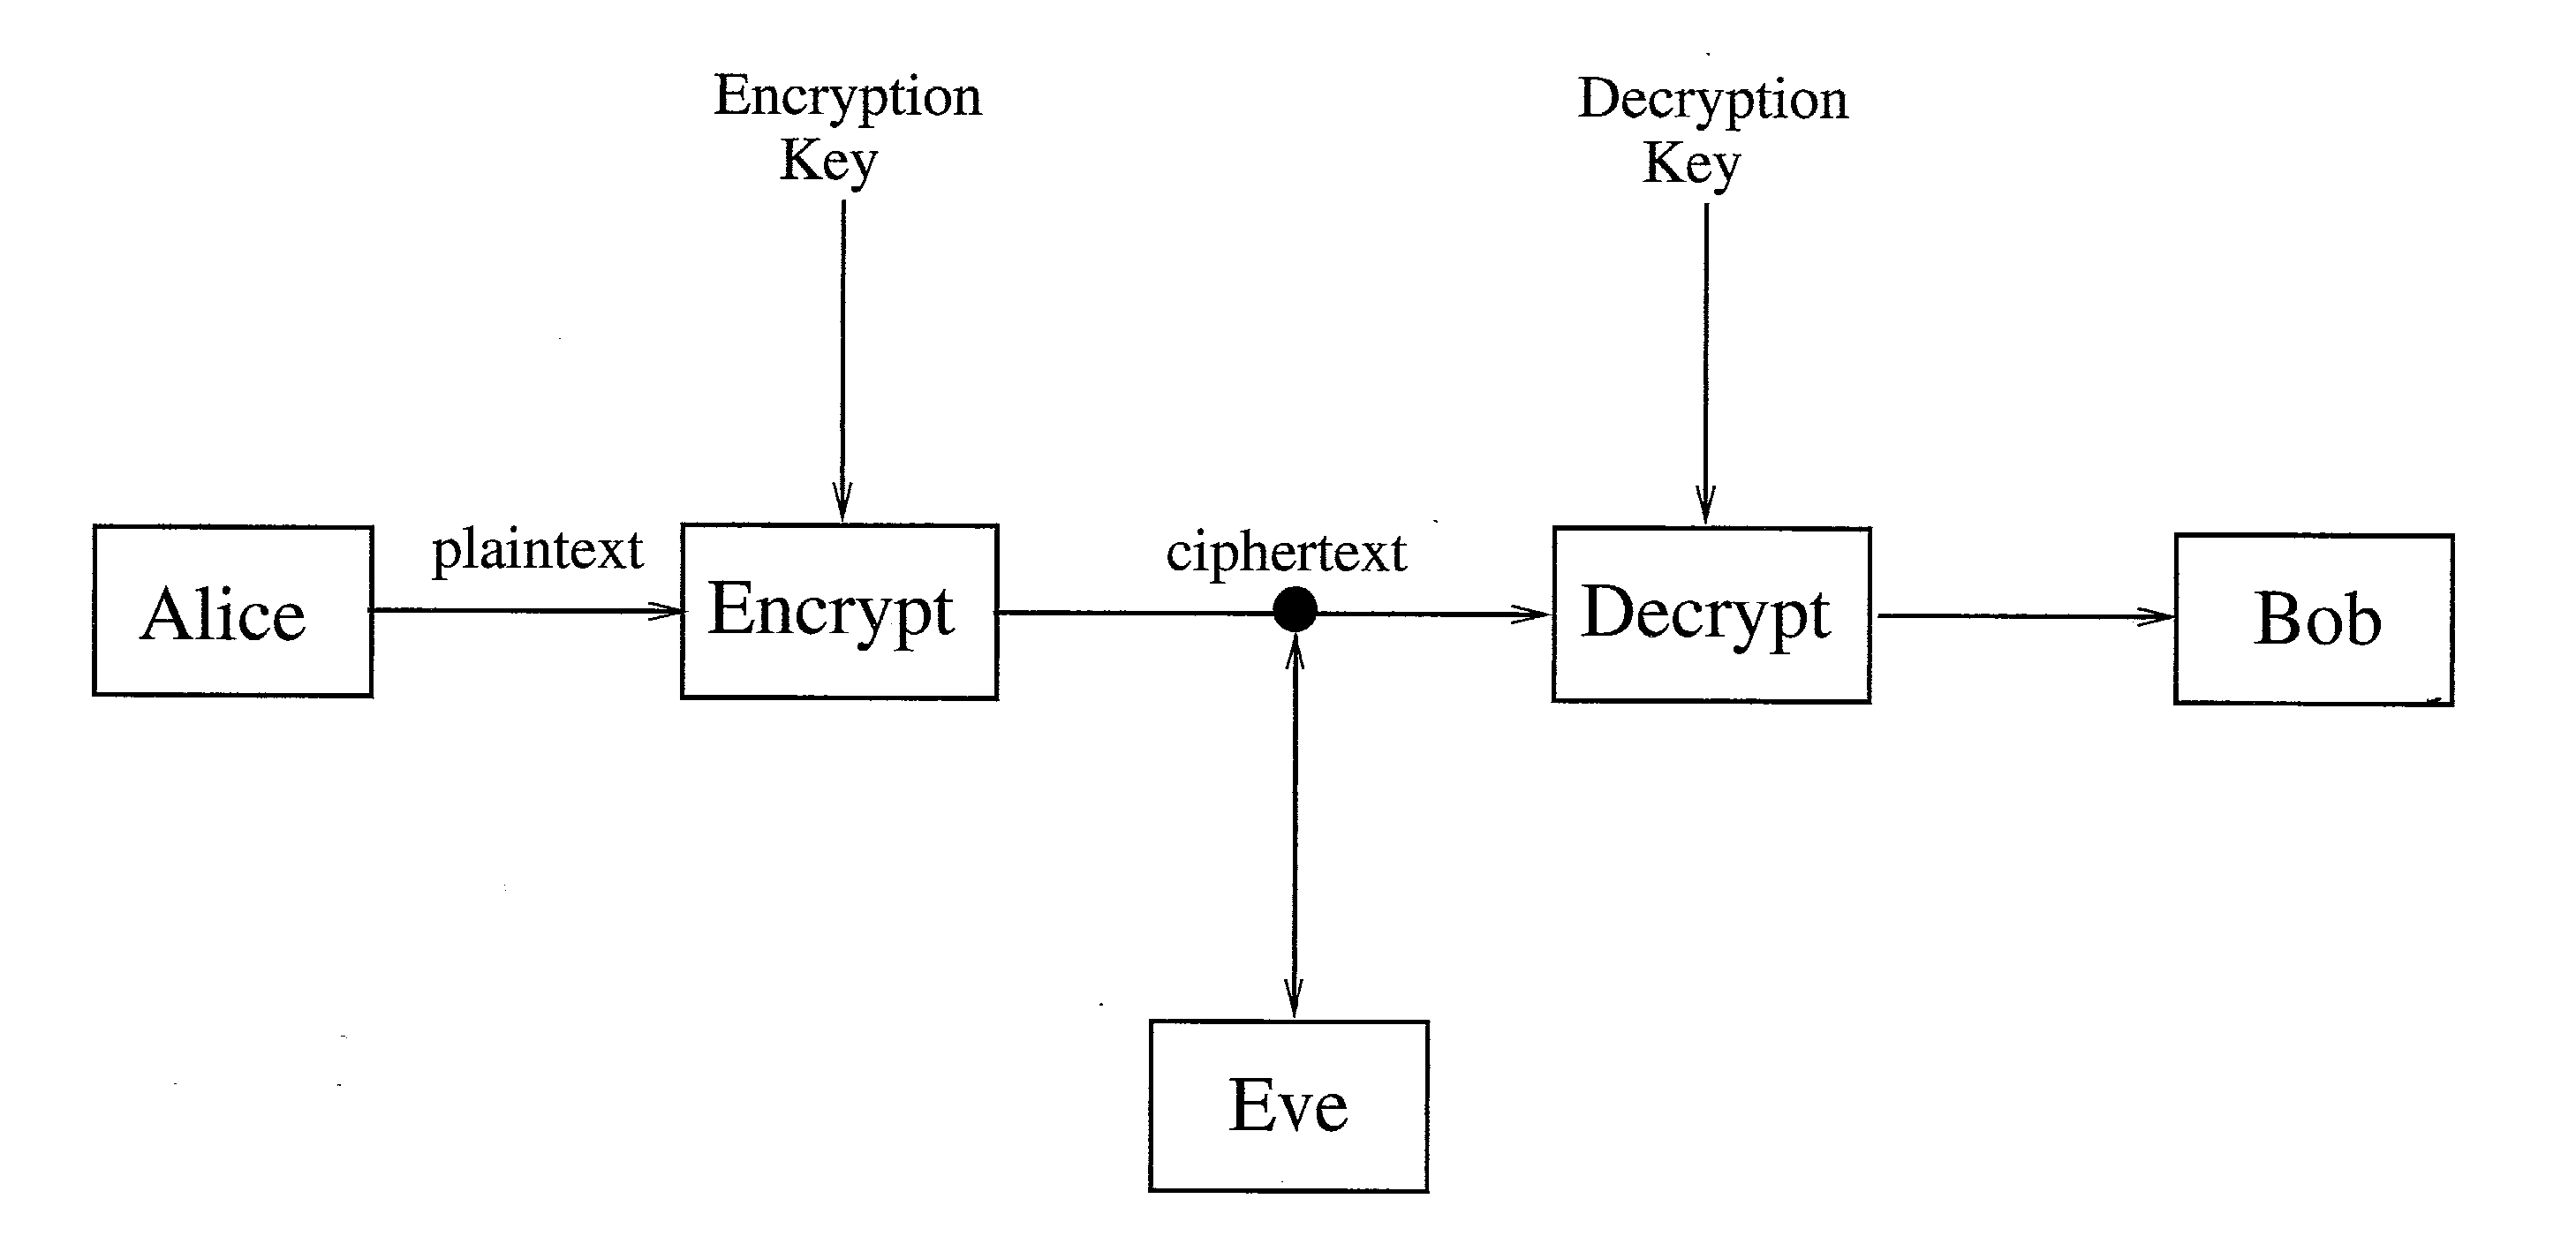
\includegraphics[width=120mm]{figs/basic-scenario.png}
		\caption{The Basic Comunication Scenario for Cryptography \cite{trappe-washington_intro-to-crypto}}
\end{figure}

\par This scenario is the standard example found in many different introductory
cryptography references. Numerous encryption and decryption methods, or {\em cryptosystems},
have been designed to secure the messages sent between Alice and Bob. Unfortunately,
many of these systems have been broken because of the amount of work that goes into
the study of breaking cryptosystems, called {\em cryptanalysis}. A constant battle
exists between the designers and breakers of cryptosystems. In fact, designing
strong cryptosystem typically requires knowledge of cryptography and cryptanalysis.

\par Before diving into the topic of this paper, there is an important assumption that must
be presented. When designing a cryptosystem, every cryptographer assumes {\em Kerckhoffs' principle}:
``In assessing the security of a cryptosystem, one should always assume the enemy knows the method
being used \cite{trappe-washington_intro-to-crypto}.'' The security of a cryptosystem
cannot be based on the concealment of the encryption and decryption algorithms. In practice,
the enemy can obtain the algorithms in many ways, including from the defection or capture
of people. The security must be based on the key and not the algorithm. 

\par Imagine that Alice's message to Bob is a sequence of 1's and 0's, as it would be
in the real world. Consider a cryptosystem which encrypts each bit in the sequence
separately. This would be done by what is called a {\em stream cipher}, which, according to Rueppel,
divides bit sequence into individual bits and enciphers each bit with a time-varying
function whose time-dependency is governed by the internal state of the stream cipher.
The stream cipher can also be thought of in terms of a {\em keystream} which is a
sequence of 1's and 0's the same length of the message that is added to the message
using addition in $\gftwo$ (also known as XOR). If the keystream was perfectly random,
then the cryptosystem would be unbreakable, or {\em perfectly secret}, as
discovered by Claude Shannon in his famous paper ``Communication Theory of Secrecy Systems,''
written in 1945 and published in 1949. This cryptosystem is known as the {\em one-time pad}.
Though it is perfectly secret, it can be difficult to implement because of the inability
to produce perfectly random keystreams. Developing a method to produce perfectly random
sequences is a contradiction in itself. If there is a method to produce the sequence,
then it cannot be perfectly random.

\par Though it is impossible to create perfectly random sequences, it is possible to get close.
This type of sequence is called a {\em pseudorandom sequence}. These sequences have extremely
long periods but are statistically indistinguishable from random sequences. This paper will discuss
the construction of pseudorandom sequences through the use of a particular finite state machine
called the {\em feedback with carry shift register}. It will also investigate the possibility of
incorporating {\em bent functions}, or perfectly non-linear functions, into the construction of
psuedorandom sequences in an attempt to resist synthesizing algorithms. 

\par The paper will follow this basic outline. Important properties of the $p$-adic integers
will be established and examples of different various kinds of $p$-adic integers will be given. 
Then, the finite-state machine will be introduced, followed by the definition of the feedback
with carry shift register. Finally, the boolean functions are defined and described and various
theorems and conjectures will be presented on bent functions.

\section{Boolean Functions}
\par This section will establish the definition of a {\em Boolean function} and introduce
a few different tools used to measure properties of these functions. First, the
finite field with two elements, denoted $\gftwo$, is defined. The definitions and
notations will follow those found in \cite{bk:cs09}.

% Definition of the finited field GF(2)
\par The two element field $(\gftwo,\oplus,\cdot)$ is the set $\{0,1\}$ with defined binary
operations $\oplus$ and $\cdot$, also commonly referred to as the {\em XOR} and
{\em AND} operators, respectively.
\begin{table}[h!]\label{table:GF(2)}
	\centering
	\begin{tabular}{|c|c|}
		\hline
		XOR&AND\\
		\hline
		$0\oplus0:=0$&$0\cdot0:=0$\\
		$0\oplus1:=1$&$0\cdot1:=0$\\
		$1\oplus0:=1$&$1\cdot0:=0$\\
		$1\oplus1:=0$&$1\cdot1:=1$\\
		\hline
	\end{tabular}
	\caption{Binary Operations for $\gftwo$}
\end{table}
\par It should be clear that $(\gftwo,\oplus,\cdot)$ is a commutative ring with an
identity. Additionally, the only non-zero element $1$ is it's own inverse. Therefore
$(\gftwo,\oplus,\cdot)$ is a finite field. The $n$-dimensional vector space over $\gftwo$
will be denoted by $\gftwo^n$, with the usual inner product. Components of these vectors,
the individual 1s and 0s, will be known as {\em bits}. For two vectors $x,y\in\gftwo^n$
where $x=(x_0,\cdots,x_{n-1})$ and $y=(y_0,\cdots,y_{n-1})$, the scalar product in
$\gftwo^n$ will be defined as $x\cdot y\equiv x_0\cdot y_0 \oplus \cdots \oplus x_{n-1}\cdot y_{n-1}$.

\begin{example}
	Let $a,b\in\gftwo^3$ such that $a=(1,0,1)$ and $b=(0,1,1)$ then
	\begin{align*}
		a+b      &=(1\oplus0,0\oplus1,1\oplus1)=(1,1,0) \\
		a\cdot b &=1\cdot0\oplus0\cdot1\oplus1\cdot1=1
	\end{align*}
\end{example}

\par Each vector in $\gftwo^n$ can be uniquely represented by an integer between
$0$ and $2^{n-1}$. The binary representation function $B$ is one-to-one.
\begin{equation}
	B:\gftwo^n\rightarrow\nnn\cup\{0\}\ {\rm such\ that }\ B(u)\equiv \sum_{i=0}^{n-1}u_i\cdot2^i.
\end{equation}

\par This definition of $B$ has created the convention where the {\em low bit} or
{\em least significant bit} appears on the left and the {\em high bit} or {\em most significant bit}
appears on the right. There is another notable function which counts the number of 1s in each
vector.

\begin{definition}
\label{def:Hamming}
	Let $u,v\in\gftwo^n$. Then $wt:\gftwo^n\rightarrow\nnn\cup\{0\}$ is defined by
	\[
	  wt(u):=\sum_{i=0}^{n-1}u_i
	\]
	and $d:\gftwo^n\times\gftwo^n\rightarrow\nnn\cup\{0\}$ is defined by
	\[
	  d(u,v):=w(u+v).
	\]
	Then $wt(u)$ is the {\em Hamming\ weight} of $u$ and $d(u,v)$ is the
	{\em Hamming\ distance} between $u$ and $v$.
\end{definition}

\begin{remark}
	The Hamming weight of a vector $u\in\gftwo^n$ is the number of 1s in the vector, and the
	Hamming distance between two vectors $u,v\in\gftwo^n$ is the number of bit differences
	between the two vectors.
\end{remark}

\begin{example}
	Let $a,b,c\in\gftwo^5$ such that
	\[
	a=(0,1,1,0,1),\ b=(1,1,1,0,0),\ {\rm and}\ c=(0,0,1,1,0)
	\]
	Then,
	\begin{align*}
		wt(a)=3 &\hspace{5mm} d(a,b)=2\\
		wt(b)=3 &\hspace{5mm} d(a,c)=3\\
		wt(c)=2 &\hspace{5mm} d(b,c)=3.\\
	\end{align*}
\end{example}
	
\par Consider the sequence $(v_0,v_1,\cdots,v_{2^n-1})$ where $B(v_i)=i$. This sequences
is said to be in {\em lexicographical order}.

\par Using the convention of lexicographical ordering and the inner product in $\gftwo^n$, a
matrix can be written which captures all of the possible inner products of two vectors in
$\gftwo^n$. This is a matrix where $u_i\cdot v_j$ appears in the $i$th row and $j$th column.
This particular matrix turns out to be a {\em Hadamard matrix} which will be studied later.

\par To complete this brief discussion about the vectors in $\gftwo^n$ is the
{\em orthogonality principle} that every non-zero vector in $\gftwo^n$ is orthogonal to
exactly half of the vectors in the vectorspace.

\begin{theorem}
	\label{thm:orthogonality-principle}
	Let $u\in\gftwo^n$. Then
	\begin{align}
		\sum_{v\in\gftwo^n}(-1)^{u\cdot v} &= 2^n {\rm \ for\ } u=0 \\
		                                   &= 0 {\rm \ otherwise.}
  \end{align}
\end{theorem}

\begin{proof}
	Let $u=0\in\gftwo^n$. Then $\forall v\in\gftwo^n u\cdot v=0$, so
	$(-1)^{u\cdot v}=1$. Therefore $\sum_{v\in\gftwo^n}(-1)^{u\cdot v}=\lvert\gftwo^n\rvert=2^n$. \\

	Let $u\in\gftwo^n$ where $u\not=0$. Assume the $i$th bit of $u$ is non-zero and
	define $e_i\in\gftwo^n$ as a vector with all zero bits except for the $i$th bit which is $1$. Then
	\begin{align*}
		\sum_{v\in\gftwo^n}(-1)^{u\cdot v} &= \sum_{v\in\gftwo^n}(-1)^{u\cdot (v+e_i)} \\
		                                   &= \sum_{v\in\gftwo^n}(-1)^{u\cdot v}(-1)^{u\cdot e_i} \\
																			 &= -\sum_{v\in\gftwo^n}(-1)^{u\cdot v}.
  \end{align*}
	Therefore, $\sum_{v\in\gftwo^n}(-1)^{u\cdot v}=-\sum_{v\in\gftwo^n}(-1)^{u\cdot v}$, which implies
	$\sum_{v\in\gftwo^n}(-1)^{u\cdot v}=0$.
\end{proof}

\par When introduced to a new vector field, it is natural to begin looking at functions in
that field. The particular function of interest here will be what is known as a {\em Boolean function}.

% Definition of a Boolean Function
\begin{definition}
\label{def:boolean-function}
  Any function $f$ defined such that 
  \begin{equation}
    f:\gftwo^n\rightarrow\gftwo
  \end{equation}
  is a {\em boolean function}.\\
	\\
	The set of all Boolean function on $n$ variables will be denoted by $\mathcal{BF}_n$
\end{definition}

\par Boolean functions have been studied extensively, and there are various properties that
are used to characterize them. Before

\par Oftentimes the codomain of a boolean function represents values of true
and false. The number of boolean functions increases
extremely rapidly as the number of variables increases.

\begin{equation}
  \lvert\{\mathcal{BF}:\fff_2^n\rightarrow\fff_2\}\rvert = 2^{2^n}
\end{equation}

\par As observed by Carlet, consider the set of all boolean functions on 7 variables,
and say that one nanosecond is spent at each function to identify the function and
note some properties about it. If we visited every boolean function this way, it
would take 100 billions times the age of the universe to complete the search.
For eight variables, there are more boolean functions than there are atoms in the
universe.

\par As always, it is best to view an example. Consider the following boolean function
$f$.
\\
\\
\begin{tabular}{|c|c|c|c|c|}
  \hline
  $x_3$&$x_2$&$x_1$&$x_0$&$f(x_3,x_2,x_1,x_0)$\\
  \hline
  0&0&0&0&0\\
  0&0&0&1&1\\
  0&0&1&0&1\\
  0&0&1&1&0\\
  0&1&0&0&1\\
  0&1&0&1&0\\
  0&1&1&0&1\\
  0&1&1&1&0\\
  1&0&0&0&0\\
  1&0&0&1&0\\
  1&0&1&0&1\\
  1&0&1&1&0\\
  1&1&0&0&0\\
  1&1&0&1&0\\
  1&1&1&0&1\\
  1&1&1&1&1\\
  \hline
\end{tabular}
\\
\\
\par The function $f$ can be written as a sum of many different functions.
In particular, it is convenient to use {\em atomic boolean functions}.

\begin{definition}
  An {\em atomic boolean function} is a boolean function that equals 1 for exactly
  one input.
\end{definition}

Then every boolean function can be written as a sum of $w(f)$ standard boolean
functions. For the above example, we have $f=f_1+f_2+f_4+f_6+f_{10}+f_{14}+f_{15}$.
\\
\\
\begin{tabular}{|c|c|c|c|c|c|c|c|c|c|c|c|}
  \hline
  $x_3$&$x_2$&$x_1$&$x_0$&$f$&$f_1$&$f_2$&$f_4$&$f_6$&$f_{10}$&$f_{14}$&$f_{15}$\\
  \hline
  0&0&0&0&0&0&0&0&0&0&0&0\\
  0&0&0&1&1&1&0&0&0&0&0&0\\
  0&0&1&0&1&0&1&0&0&0&0&0\\
  0&0&1&1&0&0&0&0&0&0&0&0\\
  0&1&0&0&1&0&0&1&0&0&0&0\\
  0&1&0&1&0&0&0&0&0&0&0&0\\
  0&1&1&0&1&0&0&0&1&0&0&0\\
  0&1&1&1&0&0&0&0&0&0&0&0\\
  1&0&0&0&0&0&0&0&0&0&0&0\\
  1&0&0&1&0&0&0&0&0&0&0&0\\
  1&0&1&0&1&0&0&0&0&1&0&0\\
  1&0&1&1&0&0&0&0&0&0&0&0\\
  1&1&0&0&0&0&0&0&0&0&0&0\\
  1&1&0&1&0&0&0&0&0&0&0&0\\
  1&1&1&0&1&0&0&0&0&0&1&0\\
  1&1&1&1&1&0&0&0&0&0&0&1\\
  \hline
\end{tabular}
\\
\\
\par This makes it easy to construct the original function $f$ because
the standard boolean functions are well-known.

\begin{align*}
  f_1   &=(1\oplus x_3)(1\oplus x_2)(1\oplus x_1)x_0\\
        &=x_0 \oplus x_1x_0 \oplus x_2x_0 \oplus x_2x_1x_0 \oplus x_3x_0 \oplus x_3x_1x_0
        \oplus x_3x_2x_0 \oplus x_3x_2x_1x_0\\
  f_2   &=(1\oplus x_3)(1\oplus x_2)x_1(1\oplus x_0)\\
  f_4   &=(1\oplus x_3)x_2(1\oplus x_1)(1\oplus x_0)\\
  f_6   &=(1\oplus x_3)x_2x_1(1\oplus x_0)\\
  f_{10}&=x_3(1\oplus x_2)x_1(1\oplus x_0)\\
  f_{14}&=x_3x_2x_1(1\oplus x_0)\\
  f_{15}&=x_3x_2x_1x_0\\
\end{align*}

\par Rather than continuing the computation and finding the polynomial for the boolean function
$f$, an algorithm will be introduced for computing the polynomial coefficients for any boolean
function.

\begin{theorem}
  For a boolean function $f$ of the form $f(x)=\bigoplus_{I\in\mathcal{P}(N)}a_Ix^I$, 
  \begin{equation}
    \forall I \in \mathcal{P}(N) \ \ a_I=\bigoplus_{supp(y)\subseteq I}f(y)
  \end{equation}
\end{theorem}



\section{The Ring of $N$-adic Integers}
\par The notation used in the definition of the $N$-adic numbers will follow
the same notation used by Borevich and Shafarevich in Chapter 1 of
{\bf Number Theory}.

\par In this section, the set of $N$-adic integers is shown to be a
commutative ring with an identity.
  
% Definition of N-adic integers
\begin{definition}
\label{def:N-adic}
  Let $N$ be an integer. Then the infinite integer sequence $\xn$
  determines a {\em $N$-adic integer} $\alpha$, or $\xn \rightarrow \alpha$, if
\begin{equation} \label{eq:seq}
  x_{i+1} \equiv x_i \pmod{N^{i+1}} \ \ \ \forall i \geq 0.
\end{equation}
  Two sequences $\xn$ and $\{x_n'\}$ determine the same $N$-adic integer
  if 
\begin{equation} \label{eq:equiv}
  x_i \equiv x_i' \pmod{N^{i+1}}\ \ \ \forall i \geq 0.
\end{equation}
  The {\em set of all $N$-adic integers} will be denoted by $\zzzn$.
\end{definition}

\par Ordinary integers will be called {\em rational integers} and each
rational integer $x$ is associated with a $N$-adic integer, determined
by the sequence \{$x,\ x, \ \dots, \ x,\ \dots$\}.
	
% example of equivalent sequences in Zp
\begin{example} \label{ex:equiv-seq}
  Let $\xn \rightarrow \alpha \in \zzz_3$. Then the first 5 terms of
  $\xn$ may look something like:
  \begin{align*}
    \xn = \{&1 \ , \ 1+2\cdot3 \ , \ 1+2\cdot3+1\cdot3^2 \ , \\
    &1+2\cdot3+1\cdot3^2 \ , \ 1+2\cdot3+1\cdot3^2+1\cdot3^4 \ , \ \dots\} \\
        = \{&1,7,16,16,97,\dots\}
  \end{align*}
  Then equivalent sequences to $\xn$ could begin differently for the
  first few terms:
  \begin{align*}
    \yn &= \{4,25,16,178,583,\dots\} \\
    \zn &= \{-2,-47,232,-308,97,\dots\}
  \end{align*}
  The sequences for $\yn$ and $\zn$ satisfy equation (\ref{eq:seq})
  for the first 5 terms, so they could be $N$-adic integers up to this
  point. Also, both are equivalent to $\xn$ according to the
  equivalence defined in equation (\ref{eq:equiv}).
  \begin{align*}
    &1 \equiv 4 \equiv 2 \pmod 3 \\
    &7 \equiv 25 \equiv -47 \pmod{3^2} \\
    &16 \equiv 16 \equiv 232 \pmod{3^3} \\
    &16 \equiv 178 \equiv -308 \pmod{3^4} \\
    &97 \equiv 583 \equiv 97 \pmod{3^5}
  \end{align*}
  Therefore $\xn,\yn,\zn \rightarrow \alpha$.
\end{example}

\par Because there are infinitely many sequence representations for any $N$-adic
integer, it is useful to define a canonical sequence to be used when
writing $N$-adic integers as sequences.
  
\begin{definition}
\label{def:canon}
  For a given $N$-adic integer $\alpha$, a given sequence $\an$ with
  the properties:
  \begin{enumerate}[i.]
    \item $\an \rightarrow \alpha$
    \item $\an=\{a_0, \ a_0+a_1\cdot N, \ \dots, \ a_0+\dots+a_i\cdot N^i, \ \dots\} : 0 \leq a_i < N \ \ \ \forall i \geq 0$
  \end{enumerate}
  will be called {\em canonical}. The number $a_0a_1a_2 \dots a_i \dots$
  is the {\em digit representation} of $\alpha$.
\end{definition}

% Insert example of a p-adic integer written in canonical form
\begin{example} \label{ex:canon}
  In Example \ref{ex:equiv-seq}, the sequence $\xn$ was a canonical
  sequence that determined the $N$-adic integer $\alpha$. A few more examples
  of canonical sequences determining 7-adic integers are given here:\\
  \\
 $\beta = 3164\dots$, then the canonical sequence $\{b_n\} \rightarrow \beta$ is
  \begin{align*}
    \{b_n\} &= \{3, \ 3+1\cdot7, \ 3+1\cdot7+6\cdot7^2, \ 3+1\cdot7+6\cdot7^2+4\cdot7^3, \ \dots\}\\
            &= \{3,10,304,1676,\dots\}
  \end{align*}
  $\gamma = 0164\dots$, then the canonical sequence $\{c_n\} \rightarrow \gamma$ is
  \begin{align*}
    \{c_n\} &= \{0, \ 1\cdot7, \ 1\cdot7+6\cdot7^2, \ 1\cdot7+6\cdot7^2+4\cdot7^3, \ \dots\}\\
            &= \{0,7,301,1673,\dots\}
  \end{align*}
  $\delta = 5031\dots$, then the canonical sequence $\{d_n\} \rightarrow \delta$ is
  \begin{align*}
    \{d_n\} &= \{5, \ 5, 5+3\cdot7^2, \ 5+3\cdot7^2+1\cdot7^3, \ \dots\}\\
            &= \{5,5,152,495,\dots\}.
  \end{align*}
\end{example}

\begin{definition}
  Addition and multiplication in $\zzzn$ are done term by term. \\
  Let $\alpha,\beta \in \zzzn$ and $\xn \rightarrow \alpha, \yn \rightarrow \beta$. Then,
  \begin{align*}
    \xn+\yn     &:= \{x_0+y_0, x_1+y_1, \dots\} \rightarrow \alpha+\beta\\
    \xn\cdot\yn &:= \{x_0 \cdot y_0, x_1 \cdot y_1, \dots\} \rightarrow \alpha \cdot \beta\\ 
  \end{align*}

  Define $\{0,0,0,\dots\} \rightarrow 0 \in \zzzn$ and $\{1,1,1,\dots\} \rightarrow 1 \in \zzzn$
\end{definition}

\begin{lemma}\label{lem:identity}
  For $\alpha \in \zzzn$, $\alpha+0=0+\alpha=\alpha$ and $1\cdot\alpha=\alpha\cdot1=\alpha$.
\end{lemma}
\begin{proof}
  Let $\xn\rightarrow\alpha\in\zzzn$.
  \begin{align*}
    \xn+\{0,0,\dots\}&=\{x_0+0,x_1+0,\dots,x_i+0,\dots\}\\
                     &=\{x_0,\dots,x_i,\dots\}.\\
    \{0,0,\dots\}+\xn&=\{0+x_0,0+x_1,\dots,0+x_i,\dots\}\\
                     &=\{x_0,\dots,x_i,\dots\}.
  \end{align*}
  $\xn=\xn+\{0,0,\dots\}=\{0,0,\dots\}+\xn$ implies $\alpha=\alpha+0=0+\alpha$.
  Therefore, the additive identity in $\zzzn$ is 0.

  \begin{align*}
    \xn\cdot\{1,1,\dots\}&=\{x_0\cdot 1,x_1\cdot 1,\dots,x_i\cdot 1,\dots\}\\
                         &=\{x_0,\dots,x_i,\dots\}.\\
    \{1,1,\dots\}\cdot\xn&=\{1\cdot x_0,1\cdot x_1,\dots,1\cdot x_i,\dots\}\\
                         &=\{x_0,\dots,x_i,\dots\}.
  \end{align*}
   $\xn=\xn\cdot\{1,1,\dots\}=\{1,1,\dots\}\cdot\xn$ implies $\alpha=\alpha\cdot1=1\cdot\alpha$.
  Therefore, the multiplicative identity in $\zzzn$ is 1.
\end{proof}   
% Insert examples of multiplication and addition

\par Finally, this paper defines a {\em ring} accroding to Fine, Gaglione, and Roesenberger and
shows that $\zzzn$ is a {\em commutative ring with an identity}.
\begin{definition}
\label{def:ring}
{\rm \cite{FGR-Alg-Method}}
  A {\em ring} is a set $R$ with two binary operations defined on it. These are usually
  called addition denoted by +, and multiplication denoted by $\cdot$ or juxtaposition,
  satisfying the following six axioms:
  \begin{enumerate}
    \item Addition is commutative: $a+b=b+a \ \ \forall a,b \in R$.
    \item Addition is associative: $a+(b+c)=(a+b)+c \ \ \forall a,b,c \in R$.
    \item There exists an additive identity, denoted by 0, such that $a+0=a \ \ \forall a \in R$.
    \item $\forall a \in R$ there exists an additive inverse, denoted by $-a$, such
      that $a+(-a)=0$.
    \item Multiplication is associative: $a(bc)=(ab)c \ \forall a,b,c \in R$
    \item Multiplication is left and right distributive over addition:
      \begin{align*}
        a(b+c)&=ab+ac \\
        (b+c)a&=ba+ca
      \end{align*}
      \newcounter{enumi_saved}
      \setcounter{enumi_saved}{\value{enumi}}
  \end{enumerate}
  If it is also true that
  \begin{enumerate}
      \setcounter{enumi}{\value{enumi_saved}}
    \item Multiplication is commutative: $ab=ba \ \ \forall a,b \in R$, then
      $R$ is a {\em commutative ring}.
      \setcounter{enumi_saved}{\value{enumi}}
  \end{enumerate}
  Further if
  \begin{enumerate}
      \setcounter{enumi}{\value{enumi_saved}}
    \item There exists a multiplicative identity denoted by 1 such that
      $a \cdot 1=a$ and $1 \cdot a=a \ \ \forall a \in R$, then $R$ is a
      {\em ring with an identity}.
  \end{enumerate}
  If $R$ satisfies all eight properties, then $R$ is a {\em commutative ring with
  an identity.}
\end{definition}

\begin{theorem}
  $\zzzn$ is a commutative ring with an identity.
\end{theorem}
% p-adic integer ring proof
\begin{proof}
  Let $\xn,\yn,\zn$ determine $\alpha,\beta,\gamma\in\zzzn$ respectively. Then
  \begin{enumerate}
    \item {\em Commutativity of Addition}
      \begin{align*}
            \xn+\yn&=\{x_0+y_0,\dots,x_i+y_i,\dots\} \\
                   &=\{y_0+x_0,\dots,y_i+x_i,\dots\} \\
                   &=\yn+\xn.
      \end{align*}
      $\xn+\yn \rightarrow \alpha+\beta$ and $\xn+\yn=\yn+\xn \rightarrow \beta+\alpha$.
      Therefore, by Definition \ref{def:N-adic}, $\alpha+\beta=\beta+\alpha$.
    \item {\em Associativity of Addition}
      \begin{align*}
        \xn+(\yn+\zn)&=\xn+\{y_0+z_0,\dots,y_i+z_i,\dots\} \\
                     &=\{x_0+(y_0+z_0),\dots,x_i+(y_i+z_i),\dots\} \\
                     &=\{(x_0+y_0)+z_0,\dots,(x_i+y_i)+z_i,\dots\} \\
                     &=\{x_0+y_0,\dots,x_i+y_i,\dots\}+\zn \\
                     &=(\xn+\yn)+\zn.
      \end{align*}
      Therefore, $\alpha+(\beta+\gamma)=(\alpha+\beta)+\gamma$.
    \item {\em Existence of the Additive Identity}
      \\ \\
      By Lemma \ref{lem:identity}, $0$ is the additive identity.
    \item {\em Existence of Additive Inverses}
      \\ \\
      Define $-\xn = \{p-x_0,p^2-x_1,\dots,p^{i+1}-x_i,\dots\} \rightarrow -\alpha$.
      Then
      \begin{align*}
        \xn+(-\xn)&=\{x_0+p-x_0,x_1+p^2-x_1,\dots,x_i+p^{i+1}-x_i,\dots\} \\
                  &=\{p,p^2,\dots,p^{i+1},\dots\} \\
                  &\equiv\{0,0,\dots\} \\
                  &=0.
      \end{align*}
      Therefore, $\alpha+(-\alpha)=0$.
    \item {\em Associativity of Multiplication}
      \begin{align*}
        \xn(\yn\zn)&=\xn\{y_0z_0,\dots,y_iz_i,\dots\} \\
                   &=\{x_0(y_0z_0),\dots,x_i(y_iz_i),\dots\} \\
                   &=\{(x_0y_0)z_0,\dots,(x_iy_i)z_i,\dots\} \\
                   &=\{x_0y_0,\dots,x_iy_i,\dots\}\zn \\
                   &=(\xn\yn)\zn.
      \end{align*}
      Therefore, $\alpha(\beta\gamma)=(\alpha\beta)\gamma$.
    \setcounter{enumi}{6}
    \item {\em Commutativity of Multiplication}
      \begin{align*}
        \xn\yn&=\{x_0y_0,\dots,x_iy_i,\dots\} \\
              &=\{y_0x_0,\dots,y_ix_i,\dots\} \\
              &=\yn\xn.
      \end{align*}
      Therefore, $\alpha\beta=\beta\alpha$.
    \setcounter{enumi}{5}
    \item {\em Left and right distributivity of multiplication over addition}
      \begin{align*}
        \xn(\yn+\zn)&=\xn\{y_0+z_0,\dots,y_i+z_i,\dots\} \\
                    &=\{x_0(y_0+z_0),\dots,x_i(y_i+z_i),\dots\} \\
                    &=\{x_0y_0+x_0z_0,\dots,x_iy_i+x_iz_i,\dots\} \\
                    &=\xn\yn+\xn\zn. \\
      \end{align*}
      By commutativity of multiplication,
      \begin{align*}
        (\yn+\zn)\xn&=\xn(\yn+\zn)\\
                    &=\xn\yn+\xn\zn\\
                    &=\yn\xn+\zn\xn.
      \end{align*}
      Therefore, $\alpha(\beta+\gamma)=\alpha\beta+\alpha\gamma$ and
      $(\beta+\gamma)\alpha=\beta\alpha+\gamma\alpha$.
    \setcounter{enumi}{7}
    \item {\em Existence of a multiplicative identity}
      \\ \\
      By Lemma \ref{lem:identity}, 1 is the multiplicative identity.
      \\ \\
      Properties 1 through 8 from Definition~\ref{def:ring} are satisfied,
      so $\zzzn$ is a commutative ring with an identity.
  \end{enumerate}
\end{proof}

\begin{theorem}\label{thm:units}
  An $N$-adic integer $\alpha$, which is determined by a sequence $\xn$, is
  a unit if and only if $x_0$ is relatively prime to $N$.
\end{theorem}
\begin{proof}
  Let $\alpha$ be a unit. Then there is an $N$-adic integer $\beta$ such that
  $\alpha\beta=1$. If $\beta$ is determined by the sequence $\yn$, then
  \begin{equation}\label{eq:units}
    x_iy_i\equiv1\pmod{N^{i+1}} \ \ \forall i \geq 0.
  \end{equation}
  In particular, $x_0y_0\equiv1\pmod N$ and hence $x_0\not\equiv0\bmod N$.
  Thus, $x_0$ is relatively prime to $N$.
  Conversely, let $x_0$ be relatively prime to $N$. Then $x_0\not\equiv0\pmod{N}$.
  From (\ref{eq:seq})
  \begin{align*}
    x_1 &\equiv x_0 \pmod N\\
    &\vdots \\
    x_{i+1} &\equiv x_i \pmod{N^i}. 
  \end{align*}
  Working backward, $x_{i+1} \equiv x_i \equiv \dots \equiv x_1 \equiv x_0 \pmod N$.
  Thus, $x_i$ is relatively prime to $p \ \ \forall i\geq0$, which implies
  $x_i$ is relatively prime to $N^{i+1}$. Consequently, $\forall i\geq0 \
  \exists y_i$ such that $x_iy_i \equiv 1 \pmod{N^{i+1}}$. Since
  $x_{i+1} \equiv x_i \pmod p^i$ and $x_{i+1}y_{i+1} \equiv x_iy_i \pmod{N^i}$.
  Then, $y_{i+1} \equiv y_i \pmod{N^i}$. Therefore the sequence $\yn$ determines
  some $N$-adic integer $\beta$. Because $x_iy_i \equiv 1 \pmod{N^{i+1}} \ \ \forall i \geq 0$,
  $\alpha\beta=1$. This means $\alpha$ is a unit.
\end{proof}

\par From this theorem it follows that a rational integer $a\in\zzzn$ is a unit if
and only if $a$ is relatively prime to $N$. If this condition holds, then $a^{-1}\in\zzzn$.
Then for any rational integer $b\in\zzzn$, $b/a=a^{-1}b\in\zzzn$.


\section{Shift Registers}\label{sec:shift-registers}
\par The {\it feedback with carry shift register} (or FCSR) is a type of
shift register used in stream ciphers. Though there exist attacks against
this type of shift register by itself, it is possible to combine FCSRs
together in ways that no known attacks are useful. This however does not
guarantee security because the combining of the FCSRs greatly increases the
complexity of the cryptanalysis on the stream cipher. Despite the security
challenges, the speed of an FCSR implementation is very attractive for
engineers of hardware based cryptosystems.

\par This section will be used as an introduction to finite state machines
and feedback with carry shift registers. The FCSR will be considered in the
binary case and analyzed using $\zzz_2$. This analysis is then extended to
the case when bent sequences which could be generated by FCSRs, which leads to
the main result in Section \ref{sec:Boolean Sequences}.

\subsection{Finite State Machines}
\par It is appropriate to preface the discussion about FCSRs with general finite
state machines. Solomon W. Golomb's book {\em Shift Register Sequences}
\cite{bk:g82}, written in 1967 and revised in 1982, established a definition of
finite state machines and shift registers used in much of the literature today.

\begin{definition}\label{finite-state-machine}
  A {\em finite state machine} consists of a finite collection of {\em states}
  $K$, which sequentially accepts a sequence of {\em inputs} from a finite set
  $A$, and produces a sequence of {\em outputs} from a finite set
  $B$. Moreover, there is an {\em output function} $\mu$ which computes
  the present output as a fixed function of present input and present state,
  and a
  {\em next state function} $\delta$ which computes the next states as a fixed
  function of present input and present state. In a more mathematical manner,
  $\mu$ and $\delta$ are defined such that
  \begin{eqnarray}
    \mu:K \times A \rightarrow B \quad &\mu(k_n,a_n)=b_n \\
    \delta:K \times A \rightarrow K \quad &\delta(k_n,a_n)=k_{n+1}
  \end{eqnarray}
\end{definition}

% insert table example of a finite state machine

\par The most fundamental observation by Golomb is the following proposition.
Its result guarantees the periodicity of any finite state machine with
eventually periodic input.

\begin{proposition}\label{prop:golomb-2}
  If the input sequence to a finite state machine is eventually periodic, then
  the output sequence is eventually periodic.
\end{proposition}
\begin{proof}
  Let $p$ be the period of the inputs once the machine becomes periodic at time
  $t$. Then, for $h>0$ and $c>t$, $a_c=a_{c+hp}$. Since $K$ is finite, there
  must be $r>s>t$ such that, for some $h>0$ such that,
  \[
  k_{r+1}=\delta(k_r,a_r)=\delta(k_s,a_{r+hp})=k_{s+1}.
  \]
  It should also be clear that $a_{r+i}=a_{r+i+hp}$ for $h>0$. So by induction,
  $\forall i>0$
  \[
  k_{r+i+1}=\delta(k_{r+i},a_{r+i})=\delta(k_{s+i},a_{r+i+hp})=k_{s+i+1}
  \]
  Finally, this proves $b_{r+i+1}=b_{s+i+1}$. Thus, the eventual period of this
  machine is $r-s$.
\end{proof}

\par The next object defined is called an $N$-ary $n$-stage machine. It can be
used to represent any finite state machine. It is also a natural generalization
of shift registers, so thinking of finite state machines in the context of
$N$-ary $n$-state machines will make the transition to talking about shift
registers much smoother.

\begin{definition}\label{N-ary-n-stage-machine}
  Choose $n,m,r\in\nnn$. Then define a finite state machine with the
  following sets:
  \begin{enumerate}[1.]
    \item $D=\{0,\dots,N-1\}$. This set contains the {\em $N$-ary digits} of the
      machine.
    \item $K=\{\sum_{i=0}^{n}x_iN^i:x_i\in D\}$. This set contains the
      {\em $N$-ary states} of the machine.
    \item $A=\{\sum_{i=0}^{m}y_iN^i:y_i\in D\}$. This set contains the
      {\em $N$-ary inputs} of the machine.
    \item $B=\{\sum_{i=0}^{r}z_iN^i:z_i\in D\}$. This set contains the
      {\em $N$-ary outputs} of the machine.
    \item $F=\{f_i(x_0,\dots,x_n,y_0,\dots,y_m):0\le i<n\}$. This set contains
      the {\em $N$-ary next state functions} of the machine.
    \item $G=\{g_i(x_0,\dots,x_n,y_0,\dots,y_m):0\le i<r\}$. This set contains
      the {\em $N$-ary output functions} of the machine.
  \end{enumerate}
  The next state and output are determined from the current state and input by the
  following equations:
  \begin{eqnarray}
    x_i^*=f_i(x_0,\dots,x_{n-1},y_0,\dots,y_{m-1}) \quad 0\le i<n \\
    z_i=g_i(x_0,\dots,x_{n-1},y_0,\dots,y_{m-1}) \quad 0\le i<r
  \end{eqnarray}
  This finite state machine is called an {\em $N$-ary $n$-stage machine} and
  will be denoted by $\mathcal{M}(N,n,m,r)$.
\end{definition}

\par By making the state the input to the machine as well, this machine
becomes autonomous in the sense that it no longer needs outside input. Then
each new state and output is based on the previous state of the machine. For
$N=2$, $f_i$ and $g_i$ are Boolean functions on $n+m$ variables.
A binary $n$-stage machine can be defined by $n+r$ Boolean functions each
on $n+m$ variables.

\subsection{Feedback with Carry Shift Registers}

\par In the set of autonomous finite state machines is a type of machine
called a {\it shift register}. The variables making up the state of a shift
register pass their values directly to the next variable in the state until
the value is pushed out of the register as the output.

\begin{definition}\label{def:shift-register}
  Let $\mathcal{M}(2,n,-1,0)$ be an binary $n$-stage machine with no input
  and exactly 1 output value. Also, let $g,f_i\in\BF_n$ where the states
  $(x_0,\cdots,x_{n-1})$ are the domain of $g$ and $f_i$, $f_i(x)=x_{i+1}$ for
  $0\leq i \leq n-2$, and $g(x)=x_0$. This type of machine will be called an {\it
  $n$-stage binary shift register} denoted by $\mathcal{SR}(2,n)$.
\end{definition}

\par When the function $f_{n-1}\in\BF_n$ is linear, then $\mathcal{SR}(2,n)$ is
called a {\it linear feedback shift register}. An LFSR is drawn in Figure
\ref{fig:LFSR}. This is the case where $f_{n-1}=\sum_{i=1}^nq_ix_{n-i}$ where
each $x_i,q_i \in \gftwo$. The $q_i$'s are called {\it taps}. In computer
science terms, to move forward in the sequence of states, each bit in the state
of the register shifts to the right one spot and then the newest bit enters
on the left end of the register and is the value given when each bit from
the previous state is AND'ed with its corresponding tap and then XOR'ed with
all the other AND'ed bit and taps.

\setlength{\unitlength}{1mm}
\begin{figure}[h!]
  \centering
  \begin{picture}(90,40)(-25,-25)
    %% State of the register
    \put(0,0){\framebox(10,10){$x_{n-1}$}}
    \put(10,0){\framebox(10,10){$x_{n-2}$}}
    \put(20,0){\framebox(10,10){$\dots$}}
    \put(30,0){\framebox(10,10){$x_{1}$}}
    \put(40,0){\framebox(10,10){$x_{0}$}}
    \put(50,5){\vector(4,0){10}}
    %% Taps
    \put(0,-13){\makebox(10,10){$q_1$}}
    \put(5,-8.5){\circle{9}}
    \put(10,-13){\makebox(10,10){$q_2$}}
    \put(15,-8.5){\circle{9}}
    \put(20,-13){\makebox(10,10){$\dots$}}
    \put(30,-13){\makebox(10,10){$q_{n-1}$}}
    \put(35,-8.5){\circle{9}}
    \put(40,-13){\makebox(10,10){$q_n$}}
    \put(45,-8.5){\circle{9}}
    %% Lines connecting Taps and the State of the Register
    \multiput(5,-0.2)(10,0){2}{\line(0,-6){4}}
    \multiput(35,-0.2)(10,0){2}{\line(0,-6){4}}
    %% Summer
    \put(-20,-25){\framebox(10,10){\Large $\sum$}}
    %% Lines from Taps to Summer
    \put(5,-12.8){\line(0,-6){3.5}}
    \put(15,-12.8){\line(0,-6){5.5}}
    \put(35,-12.8){\line(0,-6){8.5}}
    \put(45,-12.8){\line(0,-6){10.5}}
    \put(5,-16.3){\vector(-4,0){15}}
    \put(15,-18.3){\vector(-4,0){25}}
    \put(35,-21.3){\vector(-4,0){45}}
    \put(45,-23.3){\vector(-4,0){55}}
    %% Lines from Summer
    \put(-13,-15){\line(0,0){20}}
    \put(-13,5){\vector(4,0){13}}
    %% mod N
    \put(-13,5){\makebox(13,5){mod 2}}
  \end{picture}
  \caption{Linear Feedback Shift Register}
  \label{fig:LFSR}
\end{figure}

\par Linear feedback shift registers are well-studied in \cite{bk:g82}. By
using the Berlekamp-Massey algorithm it is possible to recover the state of
a given LFSR based on the output sequence. In fact given an LFSR output sequence
with period $2^n-1$, the Berlekamp-Massey algorithm will find a unique
minimal-length LFSR which generates this output after the first $2n$ digits have
been processed \cite{art:m69}. This algorithm is studied in more detail in
\cite{art:b06}.

\par In Figure \ref{fig:FCSR}, there is a memory cell attached to the linear
feedback shift register which adds some complexity to the register. In the
modified shift register shown in Figure \ref{fig:FCSR}, in each cycle, the
whole number quotient of $\sum_{i=1}^nq_ix_{n-i}$ is kept in the memory cell
$z$. The memory cell from the previous state of the modified shift register
is used to determined the sum modulo 2 for the newest bit in the state of
the register. A shift register modified in this way is known as a {\it
binary feedback with carry shift register}, or FCSR. For this paper, FCSRs
will only be considered in the binary case. Many of the theorems do
generalize the $N$-ary case, though sometimes it is necessar that $N$ be
prime.

\begin{figure}[h!]
  \centering
  \begin{picture}(90,40)(-40,-25)
    %% State of the register
    \put(0,0){\framebox(10,10){$x_{n-1}$}}
    \put(10,0){\framebox(10,10){$x_{n-2}$}}
    \put(20,0){\framebox(10,10){$\dots$}}
    \put(30,0){\framebox(10,10){$x_{1}$}}
    \put(40,0){\framebox(10,10){$x_{0}$}}
    \put(50,5){\vector(4,0){10}}
    %% Taps
    \put(0,-13){\makebox(10,10){$q_1$}}
    \put(5,-8.5){\circle{9}}
    \put(10,-13){\makebox(10,10){$q_2$}}
    \put(15,-8.5){\circle{9}}
    \put(20,-13){\makebox(10,10){$\dots$}}
    \put(30,-13){\makebox(10,10){$q_{n-1}$}}
    \put(35,-8.5){\circle{9}}
    \put(40,-13){\makebox(10,10){$q_n$}}
    \put(45,-8.5){\circle{9}}
    %% Lines connecting Taps and the State of the Register
    \multiput(5,-0.2)(10,0){2}{\line(0,-6){4}}
    \multiput(35,-0.2)(10,0){2}{\line(0,-6){4}}
    %% Summer
    \put(-20,-25){\framebox(10,10){\Large $\sum$}}
    %% Lines from Taps to Summer
    \put(5,-12.8){\line(0,-6){3.5}}
    \put(15,-12.8){\line(0,-6){5.5}}
    \put(35,-12.8){\line(0,-6){8.5}}
    \put(45,-12.8){\line(0,-6){10.5}}
    \put(5,-16.3){\vector(-4,0){15}}
    \put(15,-18.3){\vector(-4,0){25}}
    \put(35,-21.3){\vector(-4,0){45}}
    \put(45,-23.3){\vector(-4,0){55}}
    %% Lines from Summer
    \put(-13,-15){\line(0,0){20}}
    \put(-13,5){\vector(4,0){13}}
    \put(-17,-15){\line(0,0){20}}
    \put(-17,5){\vector(-4,0){13}}
    %% Memory cell z
    \put(-40,0){\framebox(10,10){$z$}}
    %% Lines from memory cell to summer
    \put(-35,0){\line(0,-6){20}}
    \put(-35,-20){\vector(4,0){15}}
    %% div 2 mod 2
    \put(-13,5){\makebox(13,5){mod $2$}}
    \put(-29.5,5){\makebox(13,5){div $2$}}
  \end{picture}
  \caption{Binary Feedback with Carry Shift Register} 
  \label{fig:FCSR}
\end{figure}

\begin{definition}\label{def:fcsr}
  Let $q_0,q_1,\dots,q_n\in\gftwo$. A {\em binary feedback with carry shift register} 
  of length $n$ with {\em taps} $q_1,\dots,q_n$ is a modified shift register
  whose states are collections
  \[
	(x_0,x_1,\dots,x_{n-1};z) \text{ where } x_i\in\gftwo \text{ and } z \in \zzz
  \]
  where $z$ is called the {\it memory cell}. The state changes according
  to the following rules:
  \begin{enumerate}[1.]
    \item Compute
      \[
      \sigma = \sum^n_{i=1}q_ia_{n-i}+z.
      \]
    \item The output is $x_0$.
    \item Then the new state $(x_0,x_1,\dots,x_{n-1};z)
      =(x_1,\dots,x_{n-1},\sigma\pmod2;\sigma(\text{div }2))$.
  \end{enumerate}
\end{definition}

\begin{lemma}\label{lem:linear-recur}
\par If the sequence $\alpha=(a_0,a_1,\cdots)$ where $a_i\in\{0,1\}$ and
$a_i\equiv x_i\pmod2$, and $\zeta=(z_{n-1},z_n,z_{n+1},\cdots)$ where each
$z_i$ is the value of the memory cell for the corresponding $x_i$, then
these two sequences are related by the following linear recurrence
\begin{equation}\label{eqn:lin-rec}
  a_k+2z_k=q_1a_{k-1}+\cdots+q_na_{k-n}+z_{k-1} \text{ for } k\geq n.
\end{equation}
\end{lemma}

\par Recall from Proposition \label{prop:golomb-2} that an FCSR must be
eventually periodic. By Proposition \label{prop:rational-periodic}, the sequence
generated by every FCSR can then be represented by a rational number in
$\zzz_2$. This rational number, or sequence generated, is entirely determined by
the initial state and the taps of the register.

\begin{proposition}{\rm \cite{art:kg97}}\label{prop:FCSR-seq}
	Let $q_1,\cdots,q_r$ be the taps, $m_{r-1}$ be the initial memory, and
	$a_{r-1},\cdots,a_1,a_0$ be the initial state of an FCSR. Define
	$q=1+\sum_{i=1}^{r}q_i2^i$ and
	\begin{equation}
		p=\left(\sum_{i=0}^{r-1}\sum_{j=0}^iq_ja_{i-j}2^i\right)-m_{r-1}2^r.
	\end{equation}
	Then the output sequence ${\bf a}$ of this FCSR is the digit representation of
	the 2-adic integer $\alpha=\sum_{i=0}^\infty a_i2^i=p/q$.
\end{proposition}
\begin{proof}
	Consider the transition from one state of the FCSR to the next. Suppose that,
	for some given state, the value of the memory is $m_{n-1}$ and that the
	contents of the register is given by the $r$ bits $a_{n-1},\cdots,a_{n-r}$.
	The next state of the register is determined by calculating
	\begin{equation}
		\sigma_n=m_{n-1}+\sum_{i=1}^rq_ia_{n-i},
	\end{equation}
	writing the new memory contents as $m_n=\sigma_n(\text{div }2)$, and writing
	the new contents of the state $a_n=\sigma_n\pmod2$. As stated in Lemma
	\ref{lem:linear-recur}, these equations may be combined into the expression
	\[
		\sigma_n=2m_n+a_n.
	\]
	It follows that
	\begin{equation}
		a_n=\sum_{i=1}^rq_ia_{n-i}+(m_{n-1}-2m_n),
	\end{equation}
	for $n\geq r$. Now, by substituting Equation write
	\begin{align*}
		\alpha&=a_0+a_1 2+\cdots+a_{r-1}2^{r-1}+\sum_{n=r}^\infty a_n2^n\\
		&=x+\sum_{n=r}^\infty\left( \sum_{i=1}^r q_ia_{n-i} \right)2^n+
  \end{align*}

	incomplete

\end{proof}

\subsection{Xu's Rational Approximation Algorithm}
\par In Andrew Klapper's book, he roughly describes Xu's rational approximation
algorithm for $\pi$-adic sequences in any ring $R$. A description of Xu's Algorithm
is presented here in the context of the ring $\zzz_2$.

\par The problem of synthesis lies in the following question: Given an eventually
periodic sequence of 0s and 1s generated by an FCSR, can you find $a$ and $b$
such that sequence generated is equivalent to digit representation of
$\frac{a}{b}\in\zzz_2$. If there are no constraints on $a$ and $b$, then 
at least a period of the sequence must be known to solve the problem. However, a
single FCSR cannot produce the digit representation of $\frac{a}{b}\in\zzz_2$ for
any $a,b\in\zzz$. As a quick example of this, consider the FCSR in Figure
\ref{fig:FCSR-4over5}. By Proposition \ref{prop:FCSR-seq}, it should be clear
that that there is a finite number of possibilities for initial states and taps
which complete determine the 2-adic integer represented by the sequence
generated.


\section{Boolean Sequences}\label{sec:Boolean Sequences}
\par The interest of this paper is stream ciphers, and there are a few
different ways to use bent functions in the implementation of a stream
cipher. Sequences generated using bent functions have nice cryptographic
properties because of their perfect nonlinearity. These sequences can be
generated multiple ways. Two easy examples are a filtering function on a
shift register producing an $m$-sequence or a shift register which uses $n$
different shift registers as input into a bent function. These two
techniques are discussed by Carlet \cite{col:c06}. Both of these
constructions use input vectors from $\gftwo^n$ in a psuedorandom order to
generate the sequence. Before scrambling the input in this way, the
sequences generated by lexicographic ordering of input vectors is
considered.

\begin{definition}
  Let $(a_n)$ be a sequence. If $T$ is the smallest integer such that
  $a_i=a_{i+T}$, then the {\em minimal\ period} of $(a_n)$ is $T$.
\end{definition}

\begin{definition}\label{def:lex-Bool-seq}
  Let $f\in\BF_n$ and $v_i\in\gftwo^n$ such that $v_i=B^{-1}(i)$ for
  $0\leq i<2^n$. Then,
  \begin{equation}
    seq(f)=(f(v_0),f(v_1),\cdots,f(v_{2^n-1}),f(v_0),\cdots)
  \end{equation}
  is a {\em lexicographical\ Boolean\ sequence}.
\end{definition}

\par Defined in this way, all lexicographical Boolean sequences have a
minimal period at most $2^n$. Using the lexicographic ordering, the Boolean
sequence generated will be repeated columns of the outputs for the Boolean
function read from the truth table of the Boolean fucntion. For example, the
lexicographic Boolean sequence of $f$ in Table \ref{tab:truth-table} is
\[
(0,1,1,0,1,0,1,0,0,0,1,0,0,0,1,1,0,1,1,0,1,0,1,0,0,0,1,0,0,0,1,1,\cdots).
\]

\begin{theorem}
  The lexicographical Boolean sequence of a Bent function has a period
  exactly $2^n$.
\end{theorem}
\begin{proof}
  For $x_i,\lambda_i\in\gftwo$ and $0\leq i\leq n-2$, define
  $(x,1)=\allowbreak(x_0,\cdots,\allowbreak x_{n-2},1)$,
  $(x,0)=\allowbreak(x_0,\cdots,\allowbreak x_{n-2},0)$, and
  $(\lambda,1)=\allowbreak(\lambda_0,\cdots,\allowbreak \lambda_{n-2},1)$.
  Suppose $f\in\BF_n$ and $seq(f)$ has a period $T=2^j<2^n$. Then,
  $f(x,0)=f(x,1)$.
  \begin{align*}
    c(\lambda,1)&=\frac{1}{2^{n/2}}
      \left(\sum_{x\in\gftwo^{n-1}}
        {(-1)^{f(x,0)+(x,0)\cdot(\lambda,1)}+
        (-1)^{f(x,1)+(x,1)\cdot(\lambda,1)}}
      \right)\\
    &=\frac{1}{2^{n/2}}
      \left(\sum_{x\in\gftwo^{n-1}}
        {(-1)^{f(x,0)}\left((-1)^{(x,0)\cdot(\lambda,1)}+
        (-1)^{(x,1)\cdot(\lambda,1)}\right)}
      \right)\\
    &=\frac{1}{2^{n/2}}
      \left(\sum_{x\in\gftwo^{n-1}}
      {(-1)^{f(x,0)}\left((-1)^{0\cdot1}+(-1)^{1\cdot1}\right)}
      \right)\\
    &=\frac{1}{2^{n/2}}
      \left(\sum_{x\in\gftwo^{n-1}}{(-1)^{f(x,0)}\cdot0}\right)\\
    &=0.
  \end{align*}
  One of the Fourier coefficients of $f$ must equal zero. Thus, $f$ cannot
  be a Bent function. Clearly, every lexicographical Boolean sequence has a
  minimal period at most $2^n$. Therefore, if $g$ is a Bent function, then
  $seq(g)$ has period exactly $2^n$.
\end{proof}

\par Boolean sequences will be considered as 2-adic exansions of rational
numbers.

\begin{definition}\label{2-adic-ex}
  Let $f\in\BF_n$ and $v_i\in\gftwo^n$ such that $v_i=B^{-1}(i)$ for
  $0\leq i<2^n$. Then,
  \begin{equation}
    \alpha_f=(f(v_0),f(v_0)+f(v_1)\cdot2,\cdots,\allowbreak
      f(v_0)+\cdots\allowbreak+f(v_i)\cdot2^i,\allowbreak\cdots)
  \end{equation}
  where $\alpha_f\in\zzz_2$ is called the {\em 2-adic\ expansion} of $f$.
\end{definition}

\begin{lemma}
  The digit representation of $\alpha_f$ is $seq(f)$.
\end{lemma}

\par Recall the Maiorana-McFarland class of Boolean functions from Section
\ref{subsec:bent-constructions}, and consider
the subset of these functions where $g(y)=0$. Then the following theorem is
true.

\begin{theorem}
  $\log_2(\alpha_{x\cdot\pi(y)})=2^{n/2}+2^{\bar{\pi}(0)}$
\end{theorem}


\nocite{*}
\bibliography{refs}{}
\bibliographystyle{amsplain}
\end{document}
